\documentclass[12pt]{article}

\usepackage{graphicx}
\usepackage{booktabs}
\usepackage{caption}
\usepackage{subcaption}
\usepackage{amsmath}
\usepackage[margin=1in]{geometry}
\usepackage{hyperref}

\graphicspath{{figures/}}

\begin{document}

% -----------------------------------------------------------------------
\section{Experiments}
% -----------------------------------------------------------------------

We evaluate the Drifting model~\cite{drifting2025} in two settings:
(1) baseline single-step image generation on ImageNet, and
(2) post-hoc energy guidance applied to the pre-trained generator.
All experiments use the \texttt{pixel\_B\_sota} checkpoint (ViT-B/16,
hidden\,=\,768, depth\,=\,12) running on CPU in pixel space (no VAE required).

% -----------------------------------------------------------------------
\subsection{Single-Step Image Generation}
% -----------------------------------------------------------------------

Figure~\ref{fig:demo_grid} shows images generated by the model for six
ImageNet classes with a single forward pass (1~NFE, CFG\,=\,1.0).
On CPU, each image takes approximately 0.7\,s after JIT compilation.

\begin{figure}[h]
  \centering
  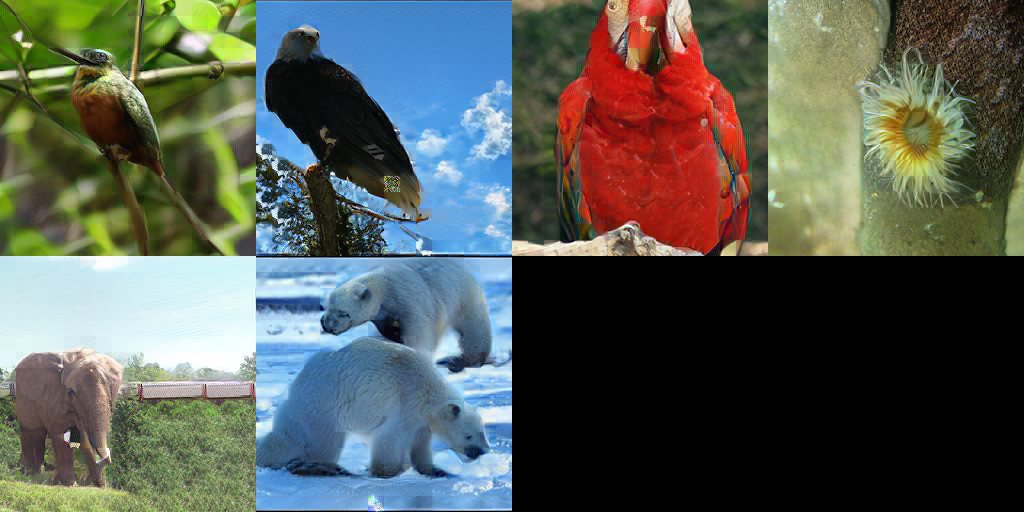
\includegraphics[width=0.65\linewidth]{grid}
  \caption{One-shot generation results ($256\times256$) for six ImageNet classes:
    jacamar (95), bald eagle (22), macaw (88), sea anemone (108),
    African elephant (386), and ice bear (296).}
  \label{fig:demo_grid}
\end{figure}

% -----------------------------------------------------------------------
\subsection{Energy Guidance}
% -----------------------------------------------------------------------

We explore steering the frozen generator with an energy function
$E(x)$ that we wish to minimise.
As a proxy task we use a red-channel preference,
$E_{\mathrm{red}}(x)=-\mathbb{E}[R-\tfrac{1}{2}G-\tfrac{1}{2}B]$,
whose gradient is closed-form and whose effect is easy to verify visually.

\paragraph{Methods.}
Two injection points are available in a single-step generator
$x = f(\varepsilon, c)$.

\begin{itemize}
  \item \textbf{Method~1 (output space).}
    Apply one gradient step directly on the generated image:
    $x' = \operatorname{clip}(x - \alpha_1 \,\nabla_x E(x) / \|\nabla_x E(x)\|_\infty,\,-1,\,1)$.
    No additional forward pass is required.

  \item \textbf{Method~2 (noise space).}
    Back-propagate through the full generator to update the input noise,
    then re-generate: $\varepsilon \leftarrow \varepsilon - \alpha_2\,
    \nabla_\varepsilon E(f(\varepsilon,c))/\|\cdot\|_2$, repeated for $T$ steps.
    Each step costs one forward and one backward pass through all 12
    transformer layers.
\end{itemize}

\paragraph{Results.}
Table~\ref{tab:red} summarises the outcome for three bird classes
under $\alpha_1{=}0.5$, $\alpha_2{=}0.3$, $T{=}5$.
Method~1 consistently reduces $E_{\mathrm{red}}$ by $\approx 0.70$, with
the R-channel mean rising by $+0.17$--$+0.25$.
Method~2, despite requiring $T$ full forward-backward passes,
achieves only $\approx 0.02$--$0.08$ reduction---roughly $10\times$--$40\times$
less than Method~1 under comparable hyperparameters.

\begin{table}[h]
  \centering
  \caption{Energy $E_{\mathrm{red}}$ and mean RGB for each class and method.
    $\Delta E$ is relative to the baseline; lower $E$ indicates a stronger red shift.}
  \label{tab:red}
  \small
  \begin{tabular}{llccccc}
    \toprule
    Class & Method & R & G & B & $E$ & $\Delta E$ \\
    \midrule
    \multirow{3}{*}{jacamar (95)}
      & Baseline     & 0.305 & 0.475 & 0.743 & $+0.609$ & ---  \\
      & Method 1     & \textbf{0.547} & 0.351 & 0.620 & $-0.123$ & $-0.732$ \\
      & Method 2     & 0.327 & 0.470 & 0.711 & $+0.527$ & $-0.082$ \\
    \midrule
    \multirow{3}{*}{bald eagle (22)}
      & Baseline     & 0.465 & 0.511 & 0.548 & $+0.128$ & ---  \\
      & Method 1     & \textbf{0.713} & 0.403 & 0.444 & $-0.580$ & $-0.708$ \\
      & Method 2     & 0.450 & 0.490 & 0.524 & $+0.113$ & $-0.015$ \\
    \midrule
    \multirow{3}{*}{macaw (88)}
      & Baseline     & 0.376 & 0.296 & 0.274 & $-0.181$ & ---  \\
      & Method 1     & \textbf{0.611} & 0.182 & 0.174 & $-0.866$ & $-0.685$ \\
      & Method 2     & 0.385 & 0.301 & 0.267 & $-0.202$ & $-0.021$ \\
    \bottomrule
  \end{tabular}
\end{table}

\paragraph{Limitations.}
Method~1 is \emph{trivial}: the update is pure pixel arithmetic decoupled
from the generator, pushing the result off the learned image manifold.
Method~2 stays on the manifold but achieves negligible energy reduction,
because the generator is ``rigid''---small perturbations in $\varepsilon$
are largely absorbed by the non-linear mapping $f$.
A single-step model has only two guidance injection points (input and output),
unlike diffusion models where guidance can be applied at every step.

\paragraph{Possible directions.}
Promising avenues include:
(1)~adding Langevin noise during $\varepsilon$ updates to stay near the
Gaussian prior while allowing larger steps, analogous to DPS~\cite{chung2022dps};
(2)~injecting guidance into intermediate transformer representations rather
than at the endpoints;
(3)~using a semantic energy (e.g.\ CLIP similarity) instead of pixel statistics.

% -----------------------------------------------------------------------
\bibliographystyle{plain}
\begin{thebibliography}{9}
\bibitem{drifting2025}
Anonymous Authors.
\newblock Generative Modeling via Drifting.
\newblock \textit{arXiv:2602.04770}, 2025.

\bibitem{chung2022dps}
H.~Chung, J.~Kim, M.~T. Mccann, M.~L. Klasky, and J.~C. Ye.
\newblock Diffusion Posterior Sampling for General Noisy Inverse Problems.
\newblock In \textit{ICLR}, 2023.
\end{thebibliography}

\end{document}
